\chapter{Tests and metrics}

After the test-bed implementation, tests about its performance and metrics were
gathered in order to understand the real project effectiveness. We performed
tests relatively two main sections: one testing the architecture overall
responsiveness and one checking the SFC implementation and efficiency.

\section{System responsiveness}

\subsection{Docker vs Virtual Box start-up measurement}

Regarding the overall system responsiveness, a metric we considered worth to 
test was the VNF start up time in a docker environment versus one virtualized 
through a common virtual machine system (in this case Virtual Box was chosen). 
To make this simulation as fair as possible, we used the same node (an 
Openstack VM with 32GB of RAM, 8 vCPU and solid state storage) and used the 
same ``boot sequence'' for both the VNFs: first we launched the Astaire 
framework, ensuring its availability to process data and then we notified the 
test machine of the successful boot. The start-up time was measured from the 
beginning of the start-up command (\verb!docker run! for Docker and 
\verb!VBoxManage -s! for Virtual Box) till the first TCP hit received by the 
test back-end (to make things as smooth as possible, \verb!netcat! was used 
to listen to incoming TCP data).

It is worth saying that Docker metrics are generally more precise than the
Virtual Box one: Docker allows to inspect the container and to gain start-up and
shutdown times with a precision of milliseconds, while to gather this 
information for VirtualBox instances we had to use the command line utility 
\verb!time!, that registered timing with a precision of hundredths of a second. 
Nonetheless, this didn't influence the test too much. To reduce possible 
outliers we performed the test $100$ times. With this $N$, the total time spent 
by the Virtual Machines to boot up was of $2021,15$ seconds, while with 
containers the same number of start ups resulted in a total of $1.638$ seconds. 
Summing up, Docker employs only the $0,08\%$ of the overall time spent for the 
test, underlining how isolating the process with a set of defined policy and 
avoiding a virtualized kernel boot-up saves a considerable amount of time.

\begin{figure}[H]
    \centering
    \begin{subfigure}[b]{0.4\textwidth}
        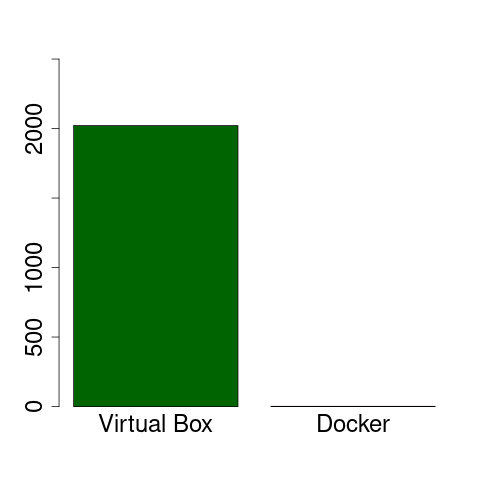
\includegraphics[scale=0.4]{docker_vs_vmBarplotGraph}
        \caption{Barplot between Virtual Box and Docker start-up times.}
        \label{chap:tests:sec:dockervsvb:img:barplot}
    \end{subfigure}
    ~
    \begin{subfigure}[b]{0.4\textwidth}
        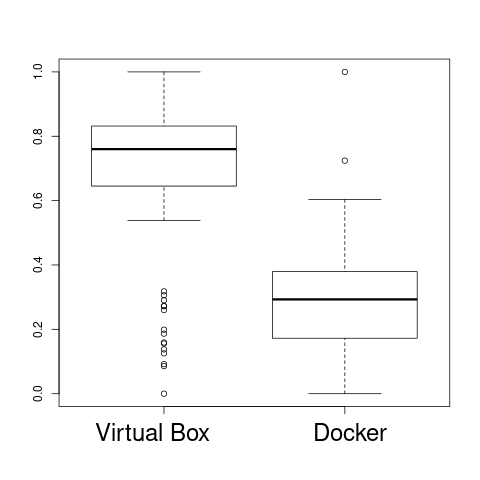
\includegraphics[scale=0.35]{docker_vs_vmBoxplotGraph}
        \caption{Boxplot between Virtual Box and Docker with values normalized 
in range $0-1$.}
        \label{chap:tests:sec:dockervsvb:img:boxplot}
    \end{subfigure}
    \caption[Virtual Box vs Docker start up comparison]{In these graphs it is
      possible to see how the total time to start up a virtual machine through
      Virtual Box is very high compared to the time required to the overall
      Docker containers to boot. A single VirtualBox instance requires on
      average 20,211 seconds to boot up, while a container requires, on average,
      only 0.016 seconds. The main reason behind this difference, as already
      explained in other parts of this thesis, it is caused by the guest's
      kernel that has to initialized itself, before starting any program. On
      Docker, instead, the kernel is the same of the host, so the only
      operations needed are to isolate the program from the rest of the OS and
      add it to the process list.}
    \label{chap:tests:sec:dockervsvb:subimg:plots}
\end{figure}


\begin{table}[t]
\centering
\resizebox{\textwidth}{!}{%
\begin{tabular}{l|c|c}
                     & \textbf{Standard deviation (seconds)} & \textbf{Average 
start up time (seconds)} \\ \hline
\textbf{Docker}      & 0.009620874                           & 0.016        \\
\textbf{Virtual Box} & 0.755                                 & 20.211
\end{tabular}%
}
\caption[Docker vs Virtual Box start up times comparison]{Docker vs Virtual Box
  start up times comparison. Is possible to see how the overall time required to
  start $100$ containers is less than the time to start one traditional virtual
  machine. The overall time required by the traditional virtualization system is
  approximately of 33 minutes, witch gives a significant insight of how much
  time is required to create and boot a virtualized environment.}
\label{my-label}
\end{table}


% The overall time required by the traditional virtualization system is
% approximately of 33 minutes, witch gives a significant insight of how much 
% time is required to create and boot a virtualized environment.


\subsection{SFC chain deploy measurement}

The previous test make us see how much Docker is faster than a traditional
virtual machine. The test, though, was performed on a single node, interacting
directly with Docker and not through the orchestrator we used in the thesis
development, Kubernetes. The following measurement will allow us to see the time
required in order to deploy an SFC of different elements in a Kubernetes
environment. The deployment consists in a Pod inside a Deployment definition
with a related Service, to simulate a real VNF. After the Pod start-up, a 
request
is made to a back-end designed to count the chain elements that have 
successfully
boot-up returning, eventually, the overall start up timing.

% TODO: missing YAML definition: [language=YAML]
%https://tex.stackexchan
%ge.com/questions/152829/how-can-i-highlight-yaml-code-in
%- a-pretty-way-with-listings
\lstinputlisting[caption={Kubernetes YAML configuration that has been used to
    simulate a single VNF deployment}, captionpos=b]{res/code/sfc_test.yaml}

\vspace{0.5cm}

\noindent As is possible to see from the YAML definition, the test involved, for
every launch (that included and $N = 100$, for a total for 1000 tests), the 
download of the container image from the Docker hub repositories. This, while 
it forced every node to delete and download the image for each test, it ensured 
consistent measurements in cases where the selected node for the deployment did 
not have the image already pulled. In addition to that, another consideration 
needs to be taken into account: when the chain consists of two or more 
elements, the container image which is used for the container deployment is the 
same for every VNF involved, thus reducing the start up time for the subsequent 
pods that reside in nodes that have already deployed one.

\begin{figure}[t]
  \centering
  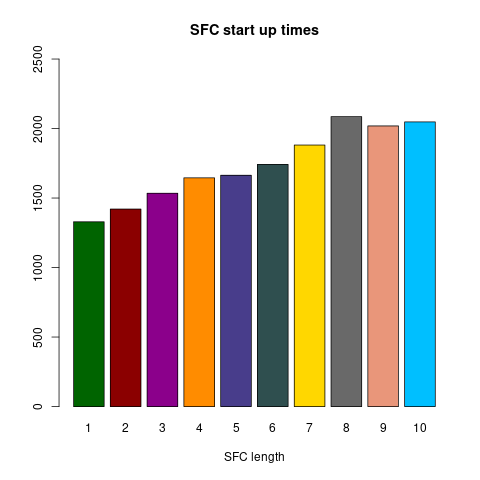
\includegraphics[scale=0.5]{sfc_startupBarplotGraph}
  \caption[SFC start-up time barplot]{SFC start-up time barplot. It is
    noticeable how there seems to be a linear correlation between the SFC
    start-up time and the SFC length, even though for the chain with eight
    elements it is possible to see that the overall deploy time is more compared
    to chains with nine and ten elements.}
  \label{chap:tests:sec:sfclength:img:barplot}
\end{figure}

\paragraph*{Kubernetes specifications}
A Kubernetes installation was performed in order to carry out the test
described above. All the machines involved (master node and minions) had the
same specifications i.e., 4GB of RAM, 2 vCPU and 10GB of SSD storage.
Nonetheless the constrained resources, absolutely far from a real Kubernetes
production environment, it is possible to notice how, even with a chain of ten
elements, the average time required to deploy an SFC is equal, if not smaller,
of the average time required to deploy a Virtual Box machine on an instance 
with 32GB of RAM, 8 vCPU and 50GB of SSD storage.

\newpage

% TODO is it worth to keep it as a long table?
\begin{longtable}[c]{c|c|c}
\textbf{SFC length} & \textbf{Standard deviation (seconds)} & \textbf{Average 
deploy time (seconds)} \\ \hline
\endhead
%
\textbf{1}          & 2.560102                   & 13.291                     \\
\textbf{2}          & 0.6301444                  & 14.207                     \\
\textbf{3}          & 1.14903                    & 15.345                     \\
\textbf{4}          & 3.592179                   & 16.453                     \\
\textbf{5}          & 0.9728132                  & 16.634                     \\
\textbf{6}          & 1.103802                   & 17.418                     \\
\textbf{7}          & 2.944699                   & 17.984                     \\
\textbf{8}          & 1.733722                   & 18.480                     \\
\textbf{9}          & 1.746296                   & 18.607                     \\
\textbf{10}         & 1.291508                   & 20.511                     \\
\caption[SFC start up time]{Table of the results. It is possible to see how the
  time required for the SFC to go up increases with the length, reaching an
  average of 20 seconds for chain of eight, nine and ten elements.}
\label{chap:tests:sec:sfclength:tab:sfcdata}\\

\end{longtable}


\paragraph*{Considerations on container start-up in Kubernetes}
Regarding the start-up times in Kubernetes is possible to denote a considerable
difference between the deployment of a SFC with only one element
(\textit{de facto} only one container) with a single container directly launched
on Docker. The difference, of many seconds, can be easily explained: the
creation of a Docker container, \textit{per se}, is quite fast compared to the
scheduling job the Kubernetes cluster has to do before launching the pod. A
Kubernetes deployment is indeed a rather complex operation than launching a
simple container. When a new deployment is launched on Kubernetes, the operation
initiate with the scheduling of a Pod. A Pod can have several lifecycle
states~\cite{kubePodLifecycle}:
\begin{description}
\item[pending:] The Pod has been accepted by the Kubernetes system, but one or
  more of the Container images has not been created. This includes time before
  being scheduled as well as time spent downloading images over the network,
  which could take a while;
\item[running:] The Pod has been bound to a node, and all of the Containers have
  been created. At least one Container is still running, or is in the process of
  starting or restarting;
\item[succeeded:] All Containers in the Pod have terminated in success, and will
  not be restarted;
\item[failed:] All Containers in the Pod have terminated, and at least one
  Container has terminated in failure. That is, the Container either exited with
  non-zero status or was terminated by the system;
\item[unknown:] For some reason the state of the Pod could not be obtained,
  typically due to an error in communicating with the host of the Pod.
\end{description}

On top of that, different conditions can affect a Pod:
\begin{itemize}
\item \verb!PodScheduled!: the Pod has been scheduled to a node;
\item \verb!Ready!: the Pod is able to serve requests and should be added to the
  load balancing pools of all matching Services;
\item \verb!Initialized!: all ``Init Containers'' have started successfully;
\item \verb!Unschedulable!: the scheduler cannot schedule the Pod right now, for
  example due to lacking of resources or other constraints.
\end{itemize}

These additional operations implicate some time overhead, that cause the
deployment of a single Pod with a single container to be way longer that the
deployment of a simple container directly from Docker.
